
\subsection{Methodology}

\subsubsection{Motivation and Definition}
This section moves beyond simple correlation to investigate linear predictive relationships between industry-specific time series and the main index. In particular, we are interested in finding industries that are "causing" the main index. Ideally, a cause should happen before its effect. Additionally, a cause should provide unique information about the future values of the effect. Finding such industries would enable us to forecast the main index. Similar considerations lead the economist Clive Granger to introduce the concept of "Granger Causality". Mathematically this is formalized by \citet{granger1969investigating} in the following way:

\begin{defn}
Let $X$,$Y$ be time-series. $X$ is said to (simple) Granger-cause $Y$ iff.    
\[
\mathrm{Var}\!\left(Y_{t+1}\middle| Y_t,\ldots,Y_1\right) \; > \; \mathrm{Var}\!\left(Y_{t+1}\middle| Y_t,\ldots,Y_1,X_t,\ldots,X_1\right)
\]
We speak of instantaneous Granger Causality iff. \[
\mathrm{Var}\!\left(Y_{t+1}\middle| Y_t,\ldots,Y_1\right) \; > \; \mathrm{Var}\!\left(Y_{t+1}\middle| Y_t,\ldots,Y_1,X_{t+1},\ldots,X_1\right)
\]

\end{defn}

\textbf{Note:} Granger causality does not claim “true” or “philosophical” causality. Instead, it identifies predictive causality, a directional and temporal relationship in which one variable systematically precedes and improves forecasts of another.

\subsubsection{Testing for Granger Causality}
To test for Granger causality, the standard approach is to compare the predictive performance of two nested linear models. First, the dependent variable $Y_t$ is regressed on its own past values up to a chosen lag order (auto-regressive model). Second, an extended model is estimated in which lagged values of another variable $X_t$ are included in addition to the lagged values of $Y_t$. If the inclusion of $X_t$ significantly improves the model’s explanatory power, then $X$ is said to Granger-cause $Y$.


Formally, the null hypothesis states that the lagged values of X do not improve the prediction of Y. The hypothesis is tested by comparing the restricted and unrestricted models using an F-test on the lagged X coefficients. If the null hypothesis is rejected at the chosen significance level, evidence for Granger causality is established. In practice, we use 5\% as the significance level for the hypothesis test and a fixed number of lags (between 1 and 6). We use the standard \textit{anova}-function from R to perform the hypothesis test.



\subsection{Results}

\subsubsection{Instantaneous Granger Causality}
We start our analysis with instantaneous Granger Causality as this concept has been longer established.
\newline

\textbf{Test with single survey question} 
\newline
The analysis was performed on every single industry classified in level 2 and level 3. For each industry, we tested the relationship between individual survey questions and the main index, applying a range of time lags from one to six periods. This multi-lag approach ensures that we capture both immediate and delayed relationships between the variables.

\begin{itemize}
    \item \textbf{Level 2}: For all 50 industries within this classification, we found that at least one survey question was instantaneous Granger Causal to the main index. This universal result at a broader industry level highlights a consistent predictive link.
    \item \textbf{Level 3}: The findings were similarly robust at the more granular level 3. Of the 61 industries analyzed, 60 demonstrated that at least one survey question was Granger Causal to the main index.
\end{itemize}





Identified Exception: A single exception was noted. The industry C2529000 - "Manufacture of containers" was the only one that did not show a Granger Causal relationship with the main index within the tested parameters.
\newline






\textbf{Significant Survey Questions} 
\newline
Given that most industries show a predictive relationship with the main index, we next identify the specific survey questions that are the most consistent and powerful predictors.. By examining the distribution of instantaneous Granger Causality across all questions, we can determine which questions are most appropriate for use in forecasting models.

\begin{figure}[H]
    \centering
    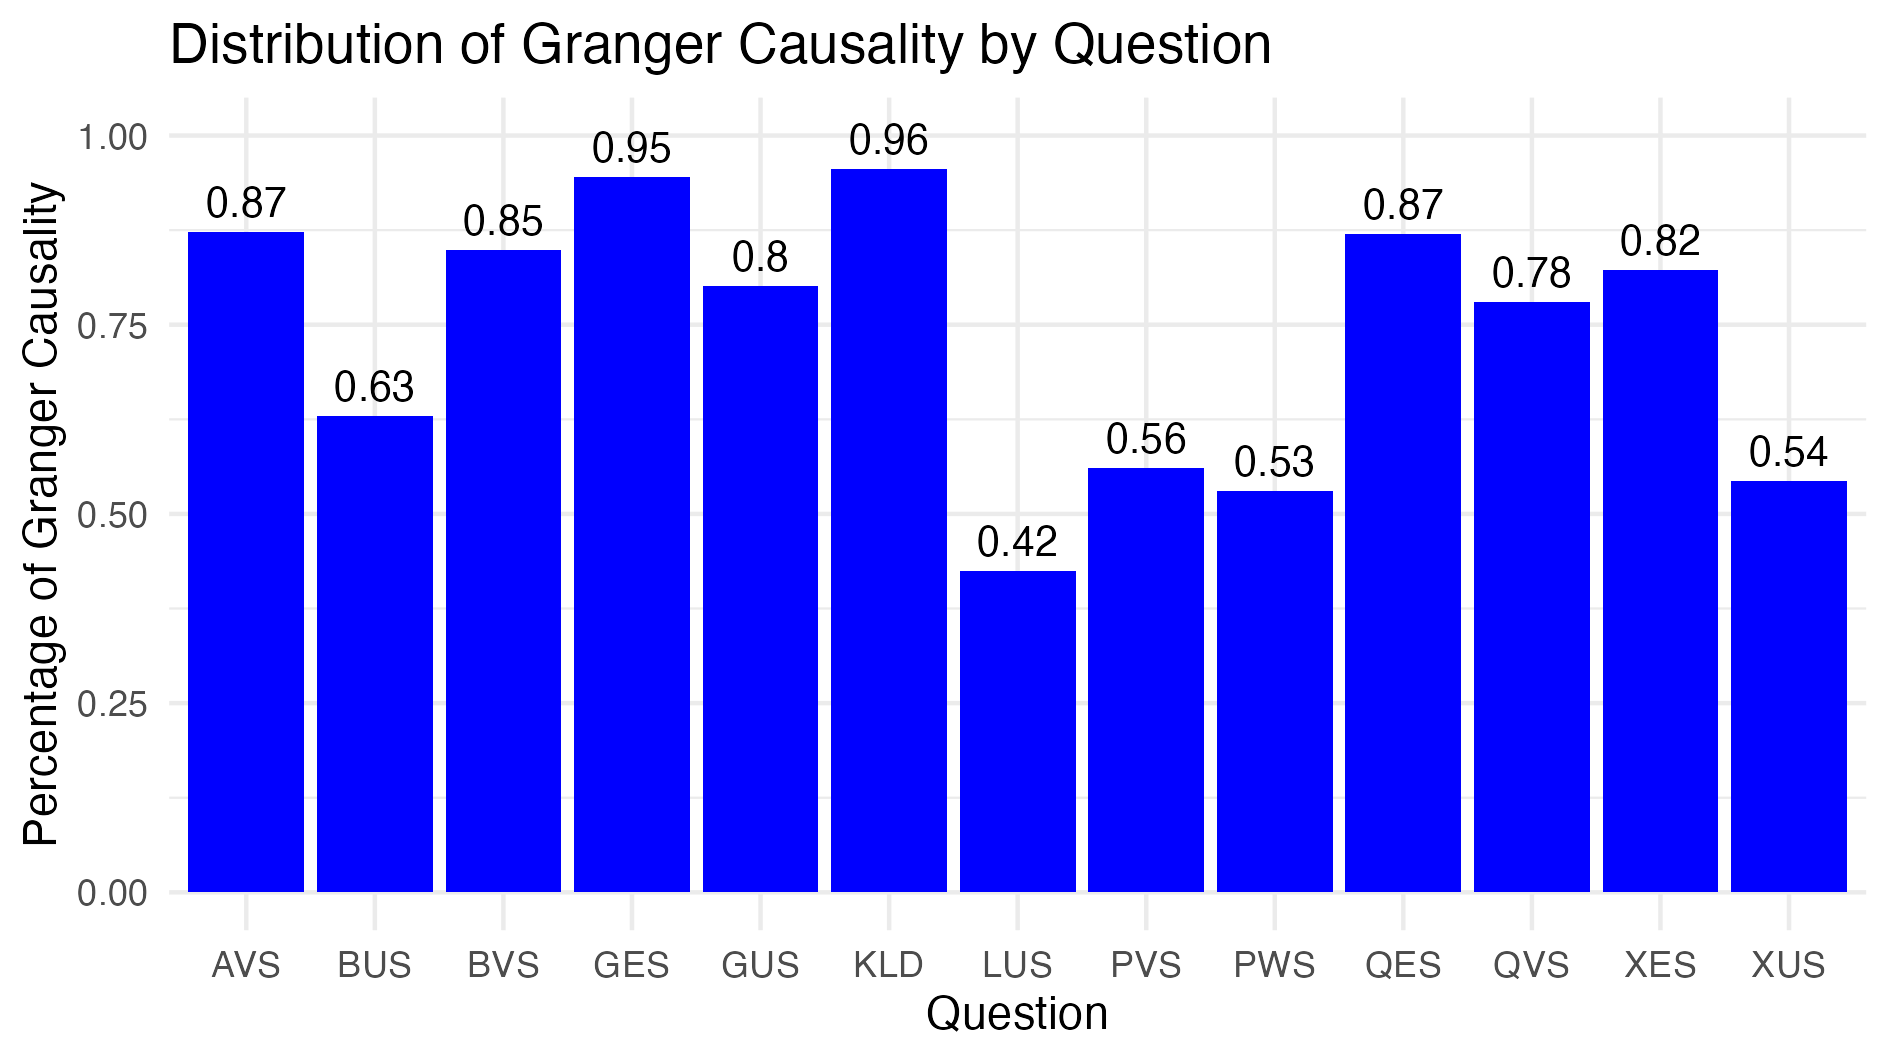
\includegraphics[width=0.9\textwidth]{DanielPlots/distribution_gc_questions_instantaneous.png}
    \caption{Distribution across questions indicating instantaneous Granger causality.}
\end{figure}

The key observations from the data are as follows:

\begin{itemize}
    \item Strongest Predictors: A few questions stand out as exceptionally reliable. The question abbreviated as KLD shows a instantaneous Granger Causal relationship in 96\% of the industries tested, followed closely by GES at 95\%. Other strong performers include AVS and QES, both at 87\%. These questions consistently provide predictive information across the vast majority of industries.

    \item Weaker Predictors: Not all questions carry the same predictive weight. The question LUS was found to be instantaneous Granger Causal in only 42\% of industries, making it the least reliable predictor in this analysis. Other questions like PVS (56\%) and PWS (53\%) are also comparatively weaker, though still predictive for a majority of industries.
\end{itemize}












\textbf{Magnitude of information gain}
\newline
To quantify the marginal contribution of industry-specific data to the performance of the forecasting model, the adjusted $R^2$ was used as the evaluation metric. The adjusted $R^2$ is utilized to determine the proportion of variance in the aggregate index that is explained by the model, adjusting for the number of predictors. The "information gain" from incorporating industry-specific data was calculated as the delta in adjusted $R^2$ between a full model containing the industry data and a reduced baseline model without it. The analysis revealed a maximum increase in adjusted $R^2$ of only 0.0212, associated with the 'Manufacture of non-industry-specific machinery' sector and it's business climate (KLD) question. This demonstrates that the marginal information gain from any single industry's data is negligible.
\begin{figure}[H]
    \centering
    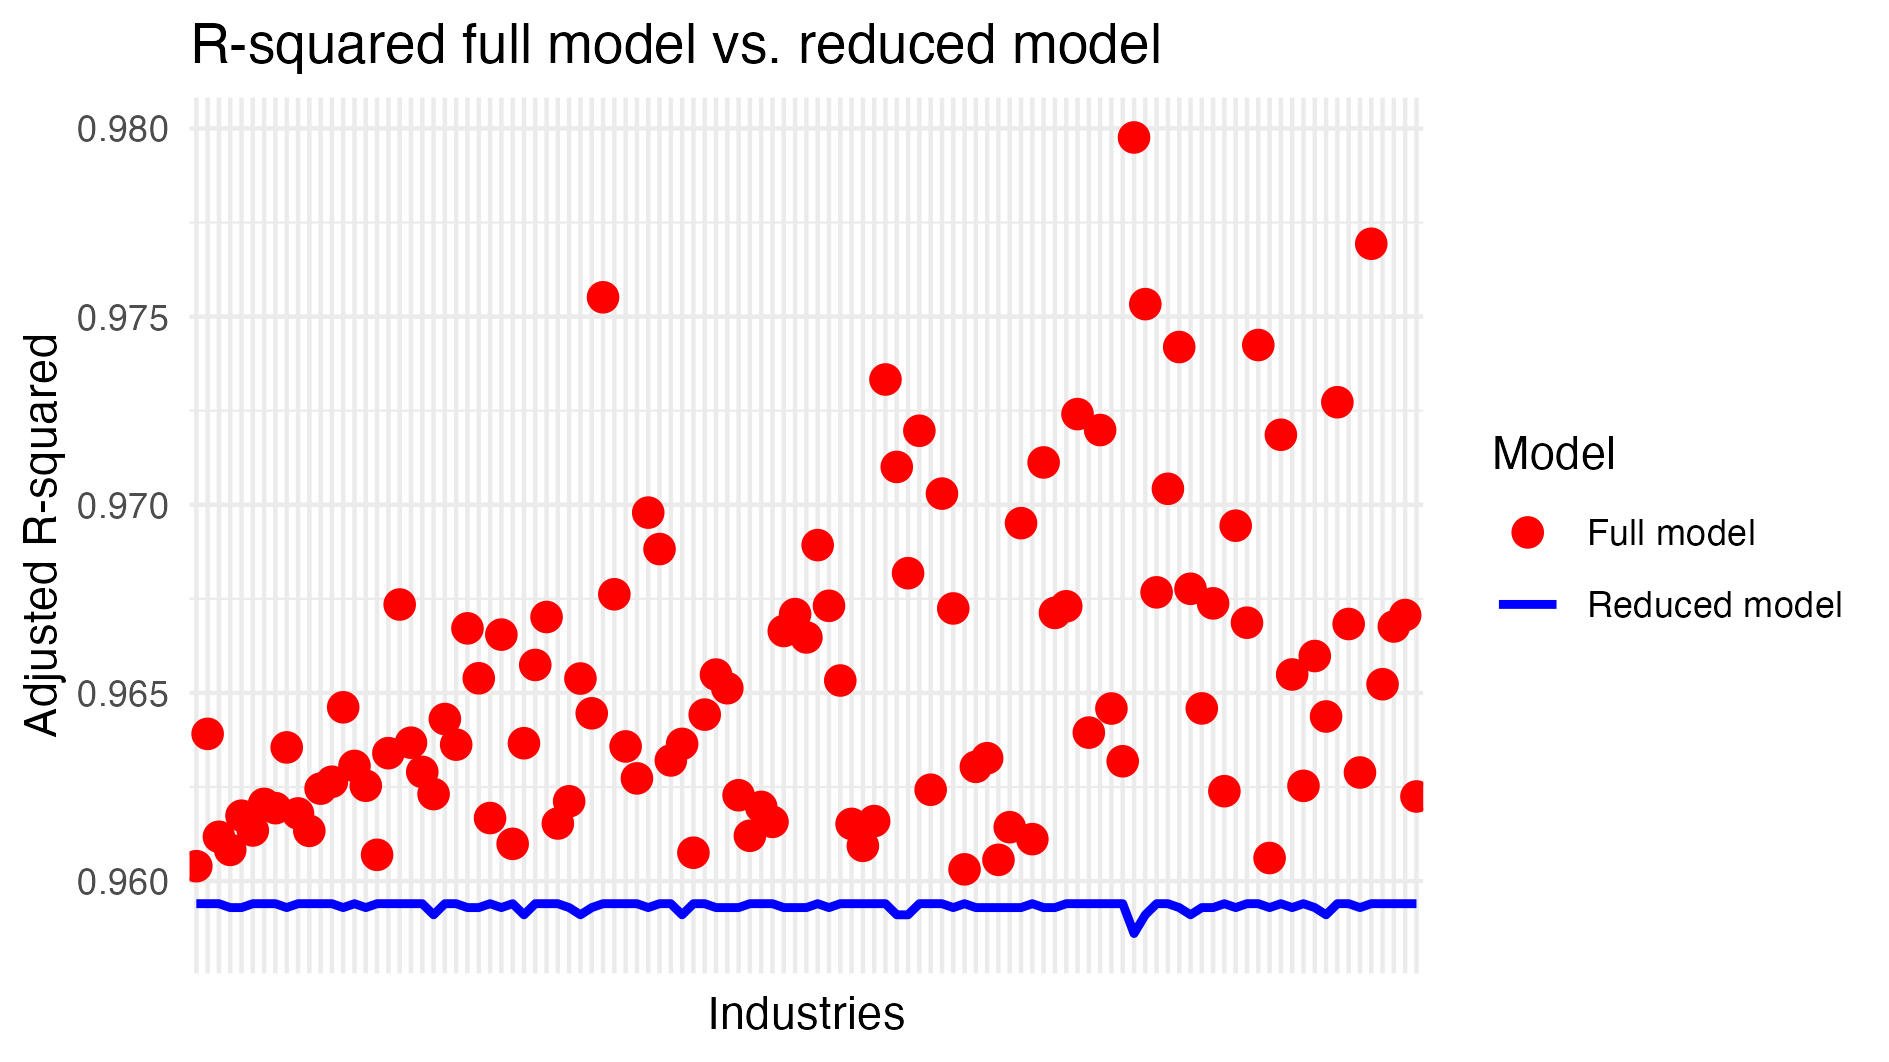
\includegraphics[width=0.9\textwidth]{DanielPlots/adj_r2_plot_instantaneous.png}
    \caption{Adjusted $R^2$ differences (univariate).}
\end{figure}



\renewcommand{\arraystretch}{1.3}
\begin{table}[H]
\centering
\begin{tabularx}{\textwidth}{X c c c}
\toprule
\textbf{Industry} & \textbf{Question} & \textbf{Lag} & \textbf{diff. adj. $R^2$} \\
\midrule
Manufacture of non-industry-specific machinery & Business climate & 3 & 0.0212 \\
Manufacture of parts and accessories for motor vehicles & Business climate & 5 & 0.0175 \\
Manufacture of plastic products & Business climate & 5 & 0.0161 \\
Manufacture of non-specialised machinery & Business climate & 6 & 0.0149 \\
Manufacture of machinery for other specific industries & Business climate & 5 & 0.0148 \\
\bottomrule
\end{tabularx}
\caption{Top 5 industries by difference in adjusted $R^2$ (univariate).}
\end{table}


Using all questions as covariates improves $R^2$, but the same industries dominate.

\renewcommand{\arraystretch}{1.3}
\begin{table}[H]
\centering
\begin{tabularx}{\textwidth}{X c c}
\toprule
\textbf{Industry} & \textbf{Lag} & \textbf{diff. adj. $R^2$} \\
\midrule
Manufacture of non-industry-specific machinery & 2 & 0.0247 \\
Manufacture of plastic products & 4 & 0.0224 \\
Manufacture of parts and accessories for motor vehicles & 6 & 0.0217 \\
Manufacture of machinery for other specific industries & 6 & 0.0204 \\
Manufacture of non-specialised machinery & 3 & 0.0191 \\
\bottomrule
\end{tabularx}
\caption{Top 5 industries by difference in adjusted $R^2$ (multivariate).}
\label{tab:top5_diff_adj_r2}
\end{table}

Visually, the business climate index for the 'Manufacture of Non-industry-specific machinery' sector exhibits a high correlation with the aggregate index but displays significantly greater amplitude in its cyclical fluctuations, with more pronounced peaks and troughs.

\begin{figure}[H]
    \centering
    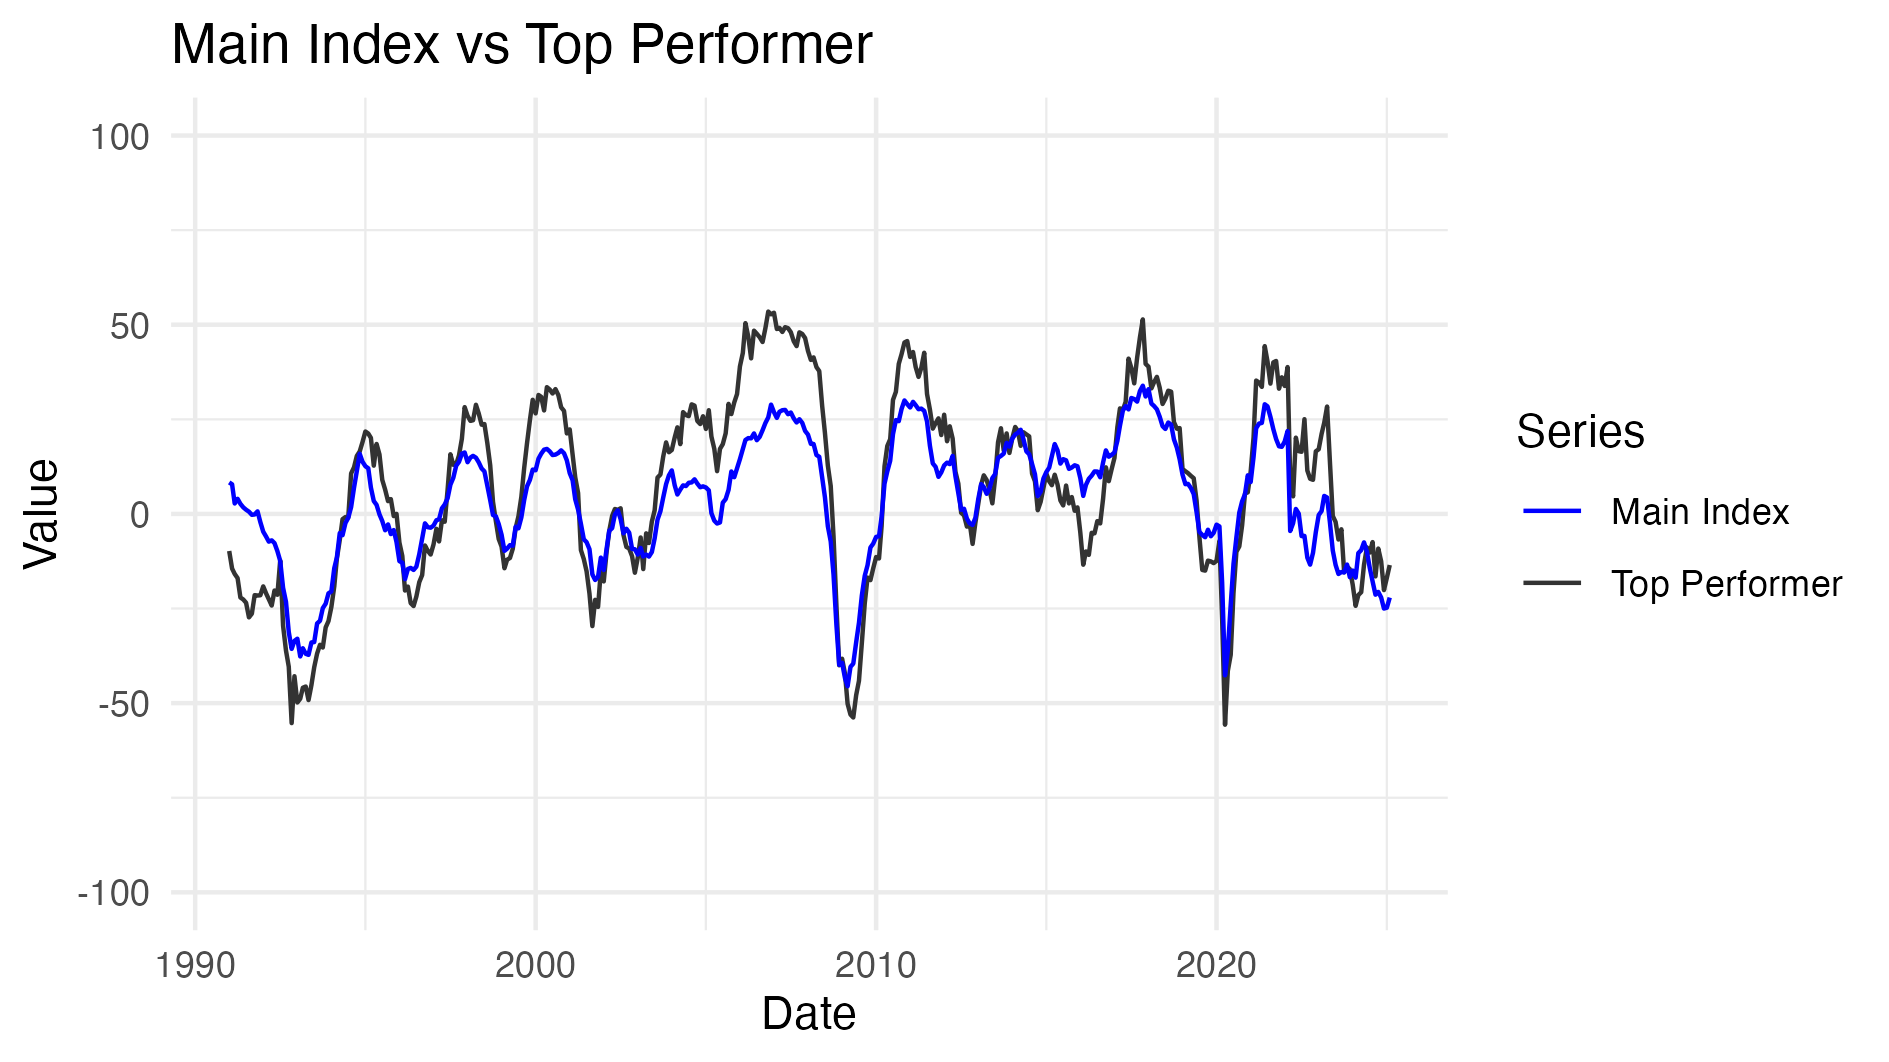
\includegraphics[width=\textwidth]{DanielPlots/main_vs_top.png}
    \caption{Main index vs.\ top-performing industry}
\end{figure}






\subsubsection{Simple Granger Causality}

Similar to the instantaneous case, the same analysis was also performed for simple Granger Causality on every single industry classified in level 2 and level 3. For each industry, we tested the relationship between individual survey questions and the main index, applying a range of time lags from one to six periods. For brevity we will highlight only the differences to instantaneous causality.
\newline





\textbf{Test with single survey question} 



\begin{itemize}
    \item \textbf{Level 2:} Only 48 out of 50 industries have at least
    one survey question that is Granger Causal to the main index.
    \item \textbf{Level 3:} Only 56 out of 61 industries have at least
    one survey question that is Granger Causal to the main index.
\end{itemize}







\textbf{Significant Survey Questions} 
\newline
Not only do the industries that are Granger Causal change but also the percentage of how often a survey question is granger causal is almost halved. Also simple Granger Causality has the most information gain with a lag of 1.

\begin{figure}[H]
    \centering
    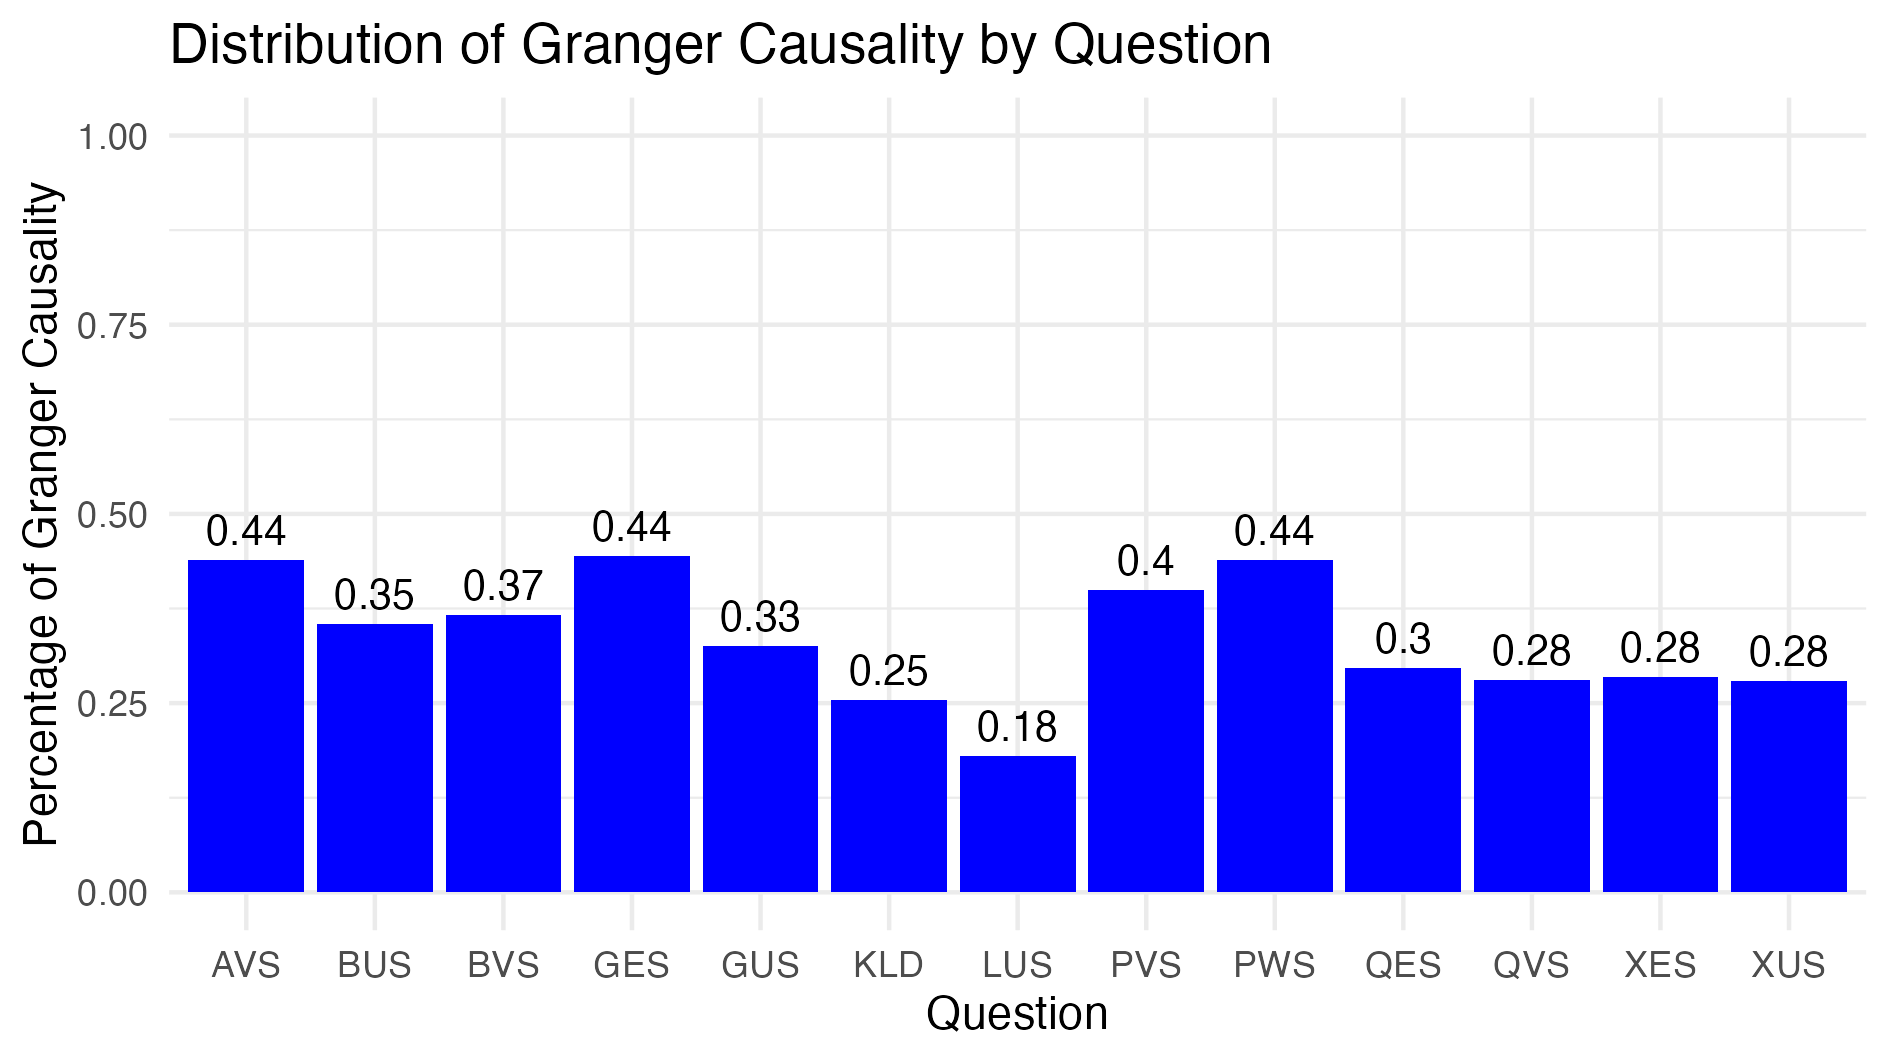
\includegraphics[width=0.9\textwidth]{DanielPlots/distribution_gc_questions_simple.png}
    \caption{Distribution across questions indicating simple Granger causality.}
\end{figure}

The key observations from the data are as follows:

    \begin{itemize}
        \item \textbf{Strongest Predictors}:  AVS, GES, and PWS at 44\% are the strongest predictors with simple Granger Causality, but are far from the 96\% maximum in instantaneous Granger Causality
        \item The predictive power of the KLD survey question for the main index is lost when relying solely on its past values. This suggests that while an industry-specific climate index may serve as a valid proxy for a contemporaneous assessment of the main index, it is insufficient for forecasting its future values.


    \end{itemize}




\textbf{Magnitude of information gain}
\newline
Compared to instantaneous Granger Causality the maximum information gain in terms of adjusted $R^2$ is even lower at 0.0073 (compared to 0.0212)
\begin{figure}[H]
    \centering
    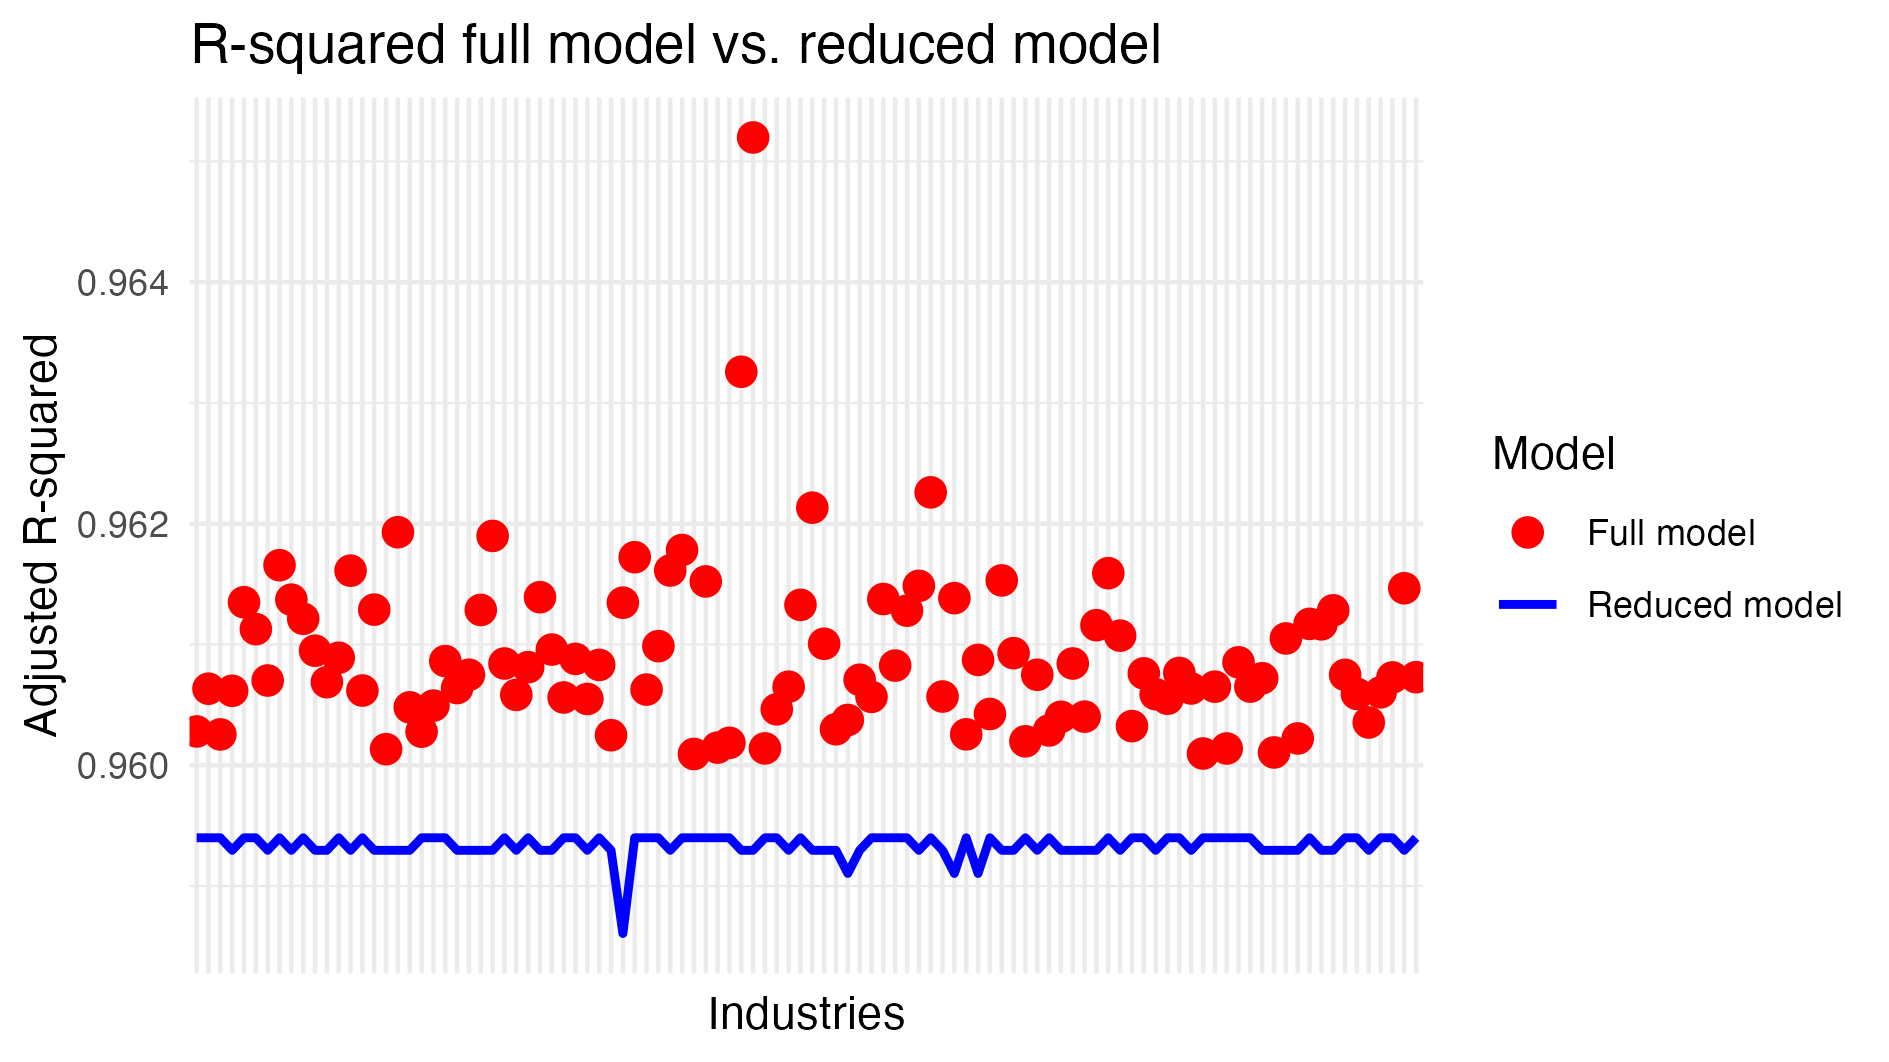
\includegraphics[width=0.8\textwidth]{DanielPlots/adj_r2_plot_simple.png}
    \caption{Adjusted $R^2$ differences (univariate).}
\end{figure}



\renewcommand{\arraystretch}{1.3}
\begin{table}[H]
\small
\centering
\begin{tabularx}{\textwidth}{X c c c}
\toprule
\textbf{Industry} & \textbf{Question} & \textbf{Lag} & \textbf{diff. adj. $R^2$} \\
\midrule
Manufacturing of tools      & business expectations      & 1   & 0.00730      \\
Manufacturing of cutting devices, tools, and locks       & business expectations      & 1   & 0.00714      \\
Manufacturing of forged, pressed, drawn, and stamped parts       & business expectations      & 1   & 0.00701      \\
Manufacturing plastic goods (C2220000)       & business expectations      & 1   & 0.00660      \\
Manufacturing of other plastic goods (C2229000)     & business expectations      & 1   & 0.00657      \\
\bottomrule
\end{tabularx}
\caption{Top 5 industries by difference in adjusted $R^2$ (univariate).}
\end{table}





\subsection{Conclusion for Granger Causality}
Statistical analysis indicates that disaggregated survey data from a vast majority of individual industries, across both 2-digit and 3-digit classification levels, is Granger causal (simple and instantaneous) to the main-index. The robustness of this finding is underscored by the observation that this relationship was absent in only a few of the more than one hundred industries analyzed. However, while these relationships are statistically significant and do possess predictive power for the aggregate index, the marginal information gain from any single industry is negligible and therefore does not meaningfully improve the model's predictive performance. Additionally an implicit requirement for Granger causality is stationarity which is violated in some survey questions and industries as outlined in \ref{stationarity}. Further analysis could examine groups of industries to predict the main index.